\subsection{Unsupervised learning}

Unsupervised learning involves learning without a coach \cite{Girolami}. The neural network must be able to "discover" patterns, features, correlations or categories in the input data set themselves and encode them in the form of output data \cite{Sanger1, Sanger2}. Neural network connections and neurons must represent a degree of self-organization.

Unsupervised learning can only be used when there is redundancy in the input data set. Without redundancy, it is impossible to discover any pattern or trait in the set of input data. From this point of view, redundancy ensures knowledge \cite{Barlow}.

The diagram below is the paradigm of unsupervised learning:

\begin{figure}[H]
  \centering
  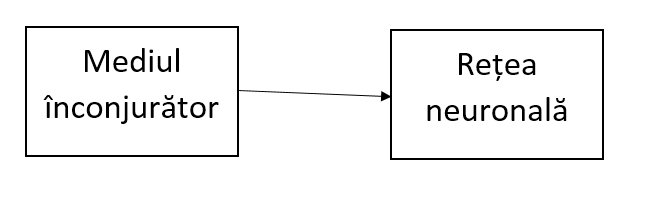
\includegraphics[width=3in]{images/diagramaInvNesupervizate.png}
  \caption {Unsupervised Learning Diagram.}
\end{figure}

In unsupervised learning, we have information about a measure of the quality of representation that the neural network needs to reach through the learning process \cite{Diamantaras}. Its parameters will be optimized for this measure. If the learning process is over, the neural network will be able to form internal representations that encode the input data features and automatically create new classes \cite{Diamantaras}.

We can use a competitive learning algorithm or a Hebbian learning algorithm for a neural network to be able to perform unsupervised learning.